\section{Fast Algorithms}

\begin{frame}
    \frametitle{Motivation I}
        \begin{columns}
            \begin{column}{0.5\textwidth}

                Consider a simple exterior scattering problem in 2D, where we can impose different boundary conditions.

                \begin{flalign*}
                    (\Delta + k^2)u^s = 0
                \end{flalign*}

            \end{column}

            \begin{column}{0.5\textwidth}
                \begin{center}
                    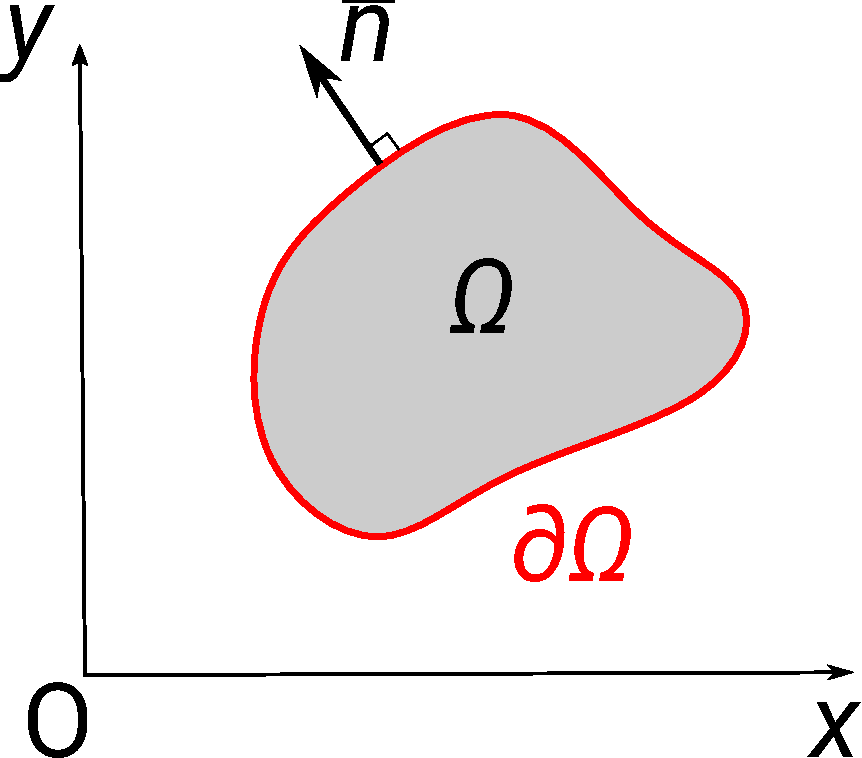
\includegraphics[width=\textwidth]{assets/laplace.pdf}
                \end{center}
            \end{column}
    \end{columns}
\end{frame}

\begin{frame}
    \frametitle{Motivation II}
        \begin{flalign*}
            (\Delta + k^2)u^s = 0
        \end{flalign*}
        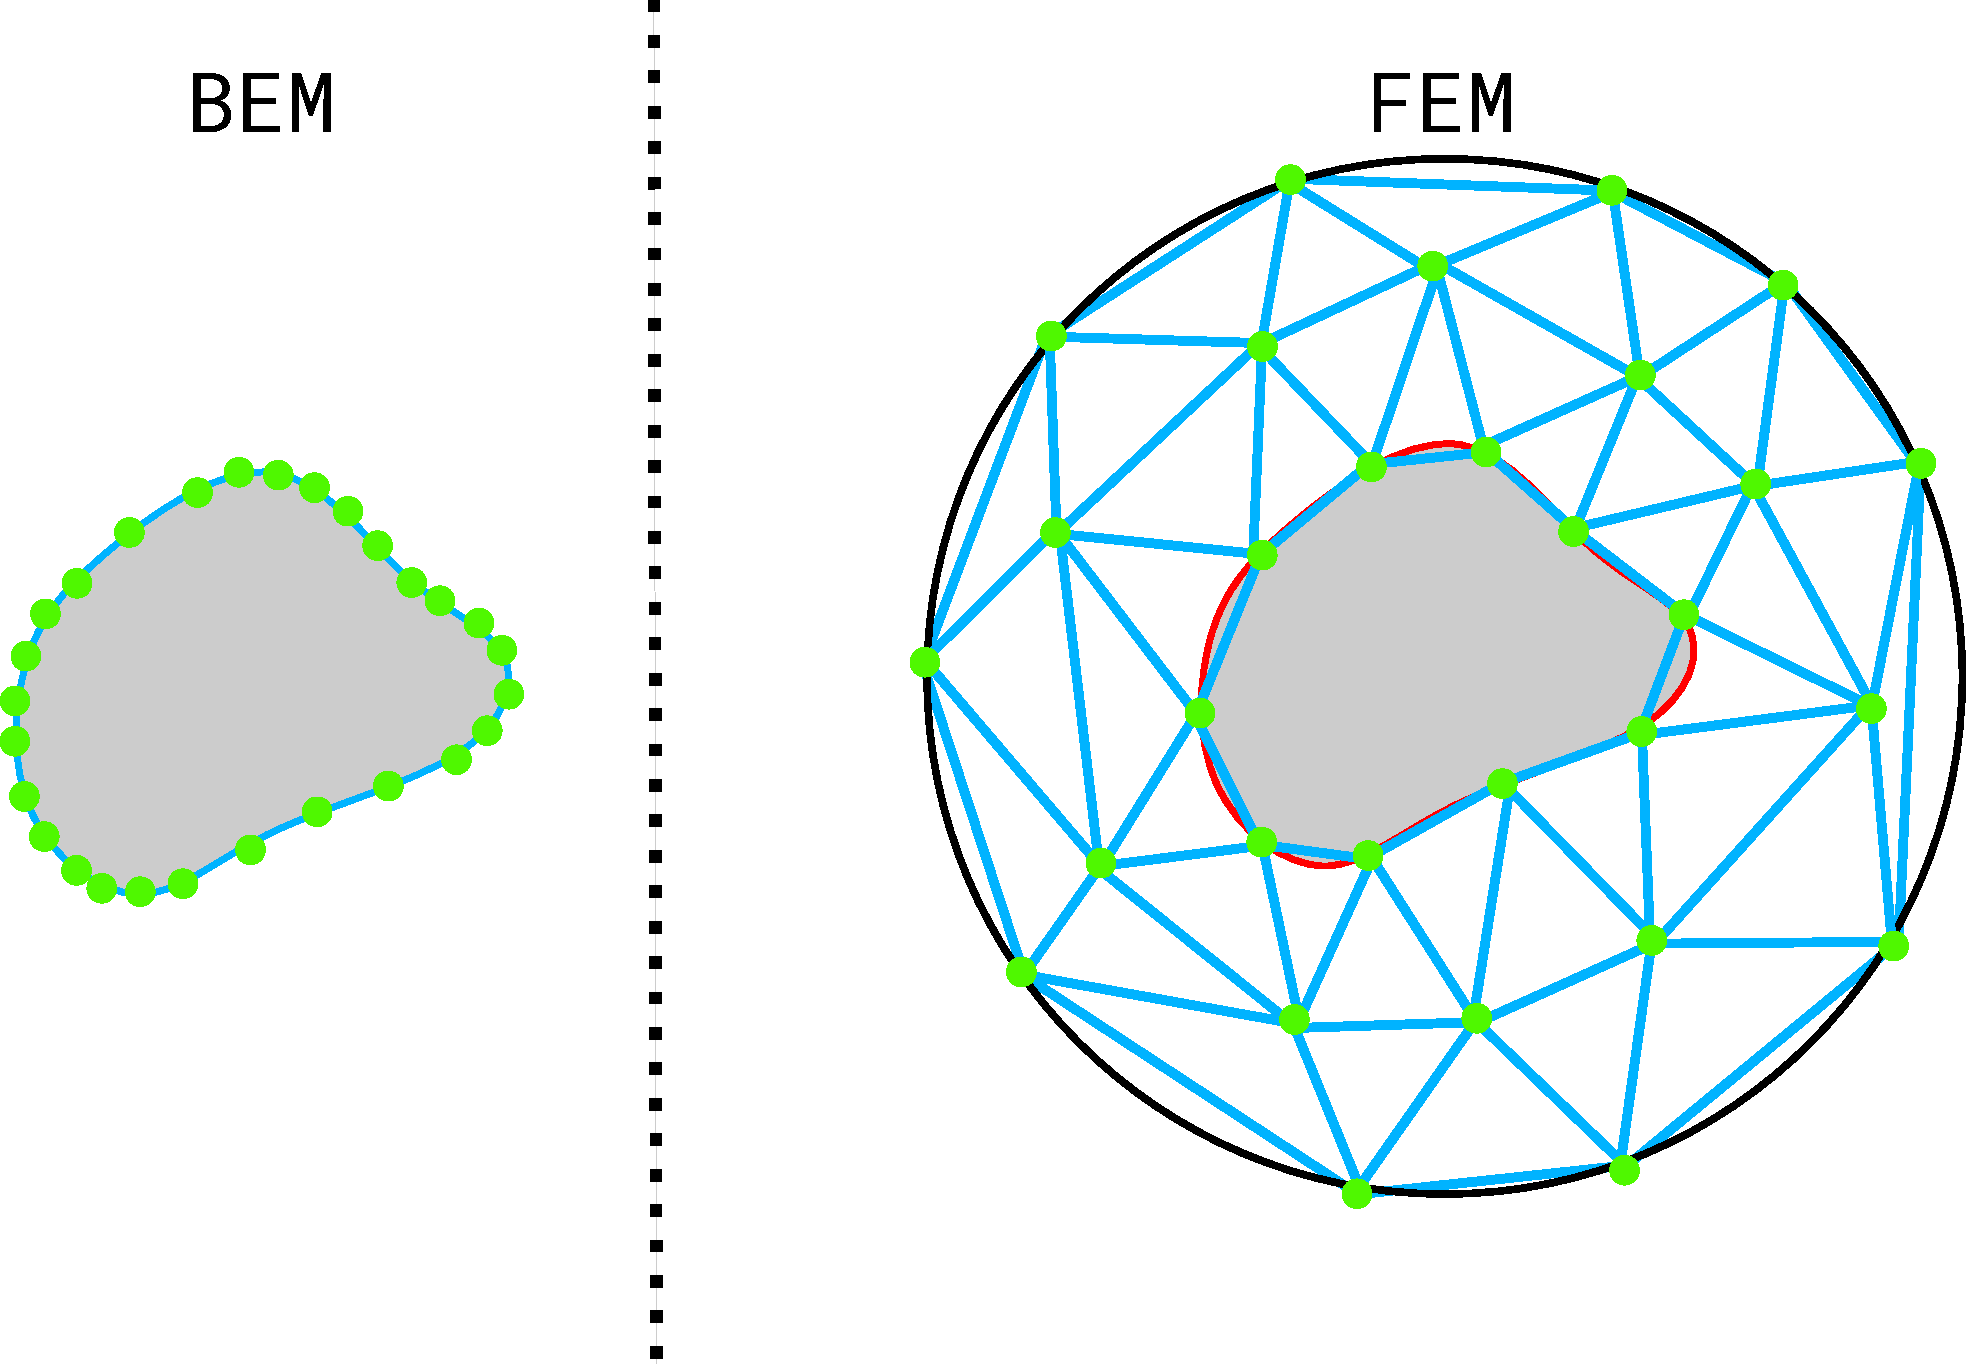
\includegraphics[width=0.9\textwidth]{assets/fem_vs_bem.pdf}
\end{frame}

\begin{frame}
    \frametitle{Motivation III}

    \begin{itemize}
        \item BEM gives us dense matrices
        \item Computational cost of naively applying to a vector is $O(N^2)$, matrix-vector product or `matvec'.
        \item Computational cost of naively inverting is $O(N^3)$, e.g LU, Gaussian Elimination, QR etc.
    \end{itemize}

    Can we take advantage of the properties of our equation to do better than this? Yes! $\rightarrow$ fast algorithms can, in the best case, reduce the application \textbf{and} inversion cost to just $O(N)$.
\end{frame}

\begin{frame}
    \frametitle{Fast Algorithms I}

    Fast algorithms enable:

    \begin{enumerate}
        \item Fast particle simulation, e.g. electrostatics and gravitation - the original application!
        \item Fast iterative methods for PDEs, e.g. Krylov subspace methods. an $O(N)$ matvec giving a final complexity of $O(N \cdot n_{\text{iter}})$.
        \item $O(N)$ Fast direct solvers for matrix inversion, better than iterative methods for problems that involve multiple right hand sides.
        \item Time-dependent problems, can solve a fixed geometry at each time step.
        \item Can solve a geometry that undergoes low-rank perturbations.
    \end{enumerate}

\end{frame}


\begin{frame}
    \frametitle{Fast Algorithms II}

    Late 1980s
    \begin{itemize}
        \item  `Analytic' Fast Multipole Methods - based on analytical multipole series expansions of kernel. $O(N)$ matvec for Laplace, Helmholtz, Stokes (Greengard and Rokhlin, 1987)
    \end{itemize}

    1990s/2000s
    \begin{itemize}
        \item  Multilevel methods (e.g. $\mathcal{H}$ and $\mathcal{H}^2$ matrices) for fast matvecs and inversion (Hackbusch, 1999), (Hackbusch and Khoromskij 2000).
        \item  `Semi-Analytic' Kernel Independent Fast Multipole Methods - based on kernel evaluations rather than analytical multipole series expansions of kernel. Easier to write generic software implementations. (Ying et al, 2004)
    \end{itemize}
    \end{frame}

    \begin{frame}

    2010s

    \begin{itemize}

        \item FMM software implementations that can process up to $O(10^6)$ of points per second (Malhotra and Biros, 2015)
        \item Fast direct solvers and software for 2D and 3D problems (Ambikasaran and Darve, 2014), (Minden et al., 2017)
    \end{itemize}

    2020s
    ...


\end{frame}


\begin{frame}
    \frametitle{From Analytic to Algebraic Fast algorithms}
    Drawbacks of analytic FMM, and analytic fast algorithms. Give sketch of semi-analytic methods, and what might be accomplished by a fully algebraic method.
\end{frame}


\begin{frame}
    \frametitle{Algebraic Fast Algorithms for Matrix Inversion}
    Fast direct solvers, overview of what they are trying to accomplish, and of course the major pros and cons.
\end{frame}


\begin{frame}
    \frametitle{Summary}
    Summarise the motivation for fast algorithms, and briefly discuss their other applications outside of integral equations.
\end{frame}

